\scanpage{27}
$K$ corps de t.f. sur $\mathbb Q$

$\overline K$ clôture algébrique.

$D$-structure sur $\overline K$ :
\[
\left\{\begin{array}{ll}
\text{a)}&\overline{\mathbb Q}\subset\overline K\\
\text{b)}&\text{pour tt courbe alg. }X\text{ sur }\overline K\text{ de type }g,\nu,
\end{array}\right.
\]
la donnée d'une discrétification de $\pi_1(X)$

$D$ structure \inserted{spéciale} \unsure{si possible} par plongt
$\varphi:\overline K\longrightarrow\mathbb C$

\deleted{\uline{Prop.} Soient $\Theta,\Theta'$ deux}

Soient $\overline K,\overline K'$ deux clôtures algébriques.
Pour tt \deleted{\unsure{K}} $K$-isom (plus gén, pour tt isom)
$\overline K\mathbin{-}\overline K'$, par transport de structure une $D$ structure
(resp. spéciale) sur $\overline K$ en définit une sur $\overline K'$.
En particulier, $\Gamma=\operatorname{Aut}(\overline K/K)$ opère sur l'ens des
discrétifications (resp. spéciales) de $\overline K$.

\uline{Prop} Soient $\overline K,\overline K'$ deux clôtures algébriques de $K$,
munies de discret. \uline{spéciales} $\Theta,\Theta'$. Alors il existe un
$K$-isom $\overline K\mathbin{-}\overline K'$ compatible avec $\Theta,\Theta'$.

\uline{Cor} Deux discrétifications spéciales sur $\overline K$ sont isomorphes
par un élémnt de $\Gamma=\operatorname{Aut}_K(\overline K)$ (et même, par un élémnt
d'un sous-groupe d'indice fini \inserted{donné} de $\Gamma$).

\uline{NB}
\diagram{\begin{tikzcd}[column sep=small]
\operatorname{Isom}_{\deleted{K}}(\overline K,\overline K')\arrow[d,phantom]&{}
\times\operatorname{Discr}(\overline K)&\operatorname{Discr}(\overline K')\\
\operatorname{Isom}_K(\overline K,\overline K')\arrow[u]&{}
\times\operatorname{Hom}(\overline K,\mathbb C)\arrow[u]\arrow[r,no head]&\operatorname{Hom}(\overline K',\mathbb C)\arrow[u]
\arrow[from=1-2,to=1-3,no head]
\end{tikzcd}}
\margin{!\quad\figure{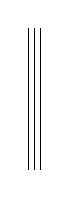
\begin{tikzpicture}\draw (0,0)--(0,1.8);\draw (.08,0)--(.08,1.8);\draw (.16,0)--(.16,1.8);\end{tikzpicture}}}
\deleted{\unsure{on tire}}\inserted{est} \unsure{le|un} commutatif.
\deleted{\unsure{$\overline K\subset\mathbb C$}}
Si $\overline K=\overline K'$, alors on se limite à
$\operatorname{Isom}_K(\overline K,\overline K')=\Gamma$ : --- \unsure{voir l'append.|cf. l'append.}
\mspage{26}
